\documentclass{llncs}
\usepackage{epsfig,amsmath,graphicx,cite,lmodern}
\usepackage{subfig,url}
\usepackage[utf8]{inputenc}
\usepackage{verbatim}

\newcommand{\zB}{z.\,B. }
\newcommand{\uA}{u.\,A. } 

\begin{document}
\mainmatter

\title{Eine Übersicht über Crossover-Operationen für genetische Algorithmen\\Seminar Organic Computing}
\titlerunning{Eine Übersicht über Crossover-Operationen für genetische Algorithmen}  % abbreviated title (for running head)

\author{Gerald Siegert\\Matrikelnummer: 1450117}
\authorrunning{Siegert} % abbreviated author list (for running head)
\tocauthor{}

\institute{Universität Augsburg\\Lehrstuhl für Organic Computing\\
\email{student@organic-computing.org}}

\maketitle


%-------------------------
\begin{abstract}
	Crossover-Operationen (CO) sind ein wesentlicher Teil von Genetischen Algorithmen (GA) und sind maßgeblich für deren Effizienz. Daher soll ein kleiner Überblick über verschiedene COs und deren Klassifizierung gegeben werden. Zunächst werden eindimensionale Re\-prä\-sen\-ta\-ti\-on\-en betrachtet. Dabei werden Darstellungen als Binärwerte, Ganzzahlen bzw. entsprechende Permutationen, Fließkommazahlen und Zeichenketten erläutert, bei welchen Problemen bzw. Anwendungsfällen welche Darstellung geeignet ist, und einige der dafür optimierten COs aufgezeigt. Ebenso betrachtet werden mehrdimensionale Re\-prä\-sen\-ta\-ti\-on\-en wie Bäume und Arrays. Es wird zudem eine kleine Über\-sicht über weitere mehrdimensionale Repräsentationen gegeben. Ebenso wird auch darauf eingegangen, wann es geeignet ist, anwendungsspezifische Co\-die\-rungen zu nutzen und anzuwenden. Ebenso werden zudem einige universell nutzbare COs aufgezeigt, die nicht an eine spezielle Repräsentation der Daten gebunden sind.
\end{abstract}

\pagebreak

\section{Einführung in genetische Algorithmen}
\label{sec:EinfGA}

Genetische Algorithmen (GA) sind genauso wie andere Evolutionäre Algorithmen im Allgemeinen aus der Biologie übernommen worden. Wie der Name schon aussagt, basieren sie auf dem Prinzip der Evolution, bei der basierend auf einer Ausgangspopulation möglicher Lösungen neue Kinder erzeugt werden, welche dann die Vorfahren in der Population verdrängen. Welche Vorfahren, oder gar die erzeugten Kinder, dabei konkret verdrängt werden, entscheidet sich basierend auf einer Fitness-Funktion, bei der die gefundenen Lösungen der Population evaluiert werden und anschließend nur die besten in der Population verweilen dürfen.

\begin{figure}
	\centering
	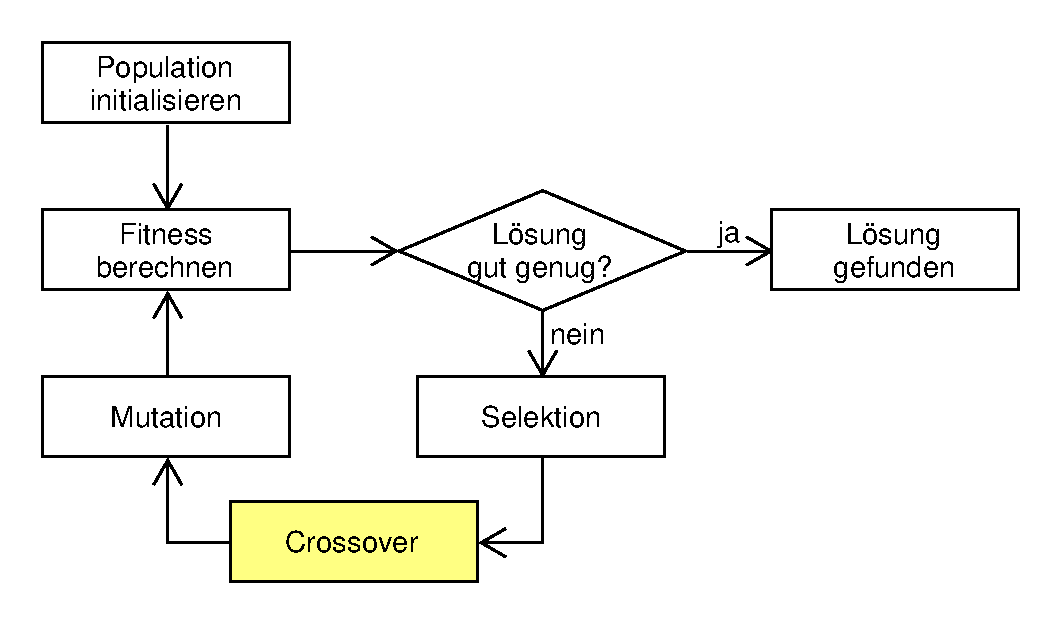
\includegraphics[width=.8\columnwidth]{./Figures/GA-Prinzip.pdf}
	\caption{Grundlegender Ablauf eines genetischen Algorithmus}
	\label{fig:abb1}
\end{figure}	

Die wichtigen Parameter eines GA selbst sind zum einen die Selektion der Gene, deren Crossover-Operationen (CO) zur Erzeugung neuer Kinder, sowie die Durch\-füh\-rung anschließender Mutationen. Maßgeblich für die Qualität und Effizienz eines GA ist dabei die in Fig. \ref{fig:abb1} markierte CO.

In dieser Seminararbeit soll daher nun ein kleiner Überblick über einige verschiedene COs gegeben werden. Nach einer Übersicht der Klassifikationen im Abschnitt \ref{sec:KlassCO} werden im Abschnitt \ref{sec:EindimRep} zuerst geeignete Anwendungen und dazugehörige COs für eindimensionale, im darauf folgenden Abschnitt \ref{sec:MehrdimRep} eine Übersicht für mehrdimensionale Repräsentationen aufgezeigt. Anschließend wird im Abschnitt \ref{sec:AnwSpezCod} ein kurzer Überblick über anwendungsspezifische Codierung, sowie im Abschnitt \ref{sec:UnivOp} über universell einsetzbare COs gegeben.

\section{Klassifizierungen von Crossover-Operationen}
\label{sec:KlassCO}

\begin{figure}
	\centering
	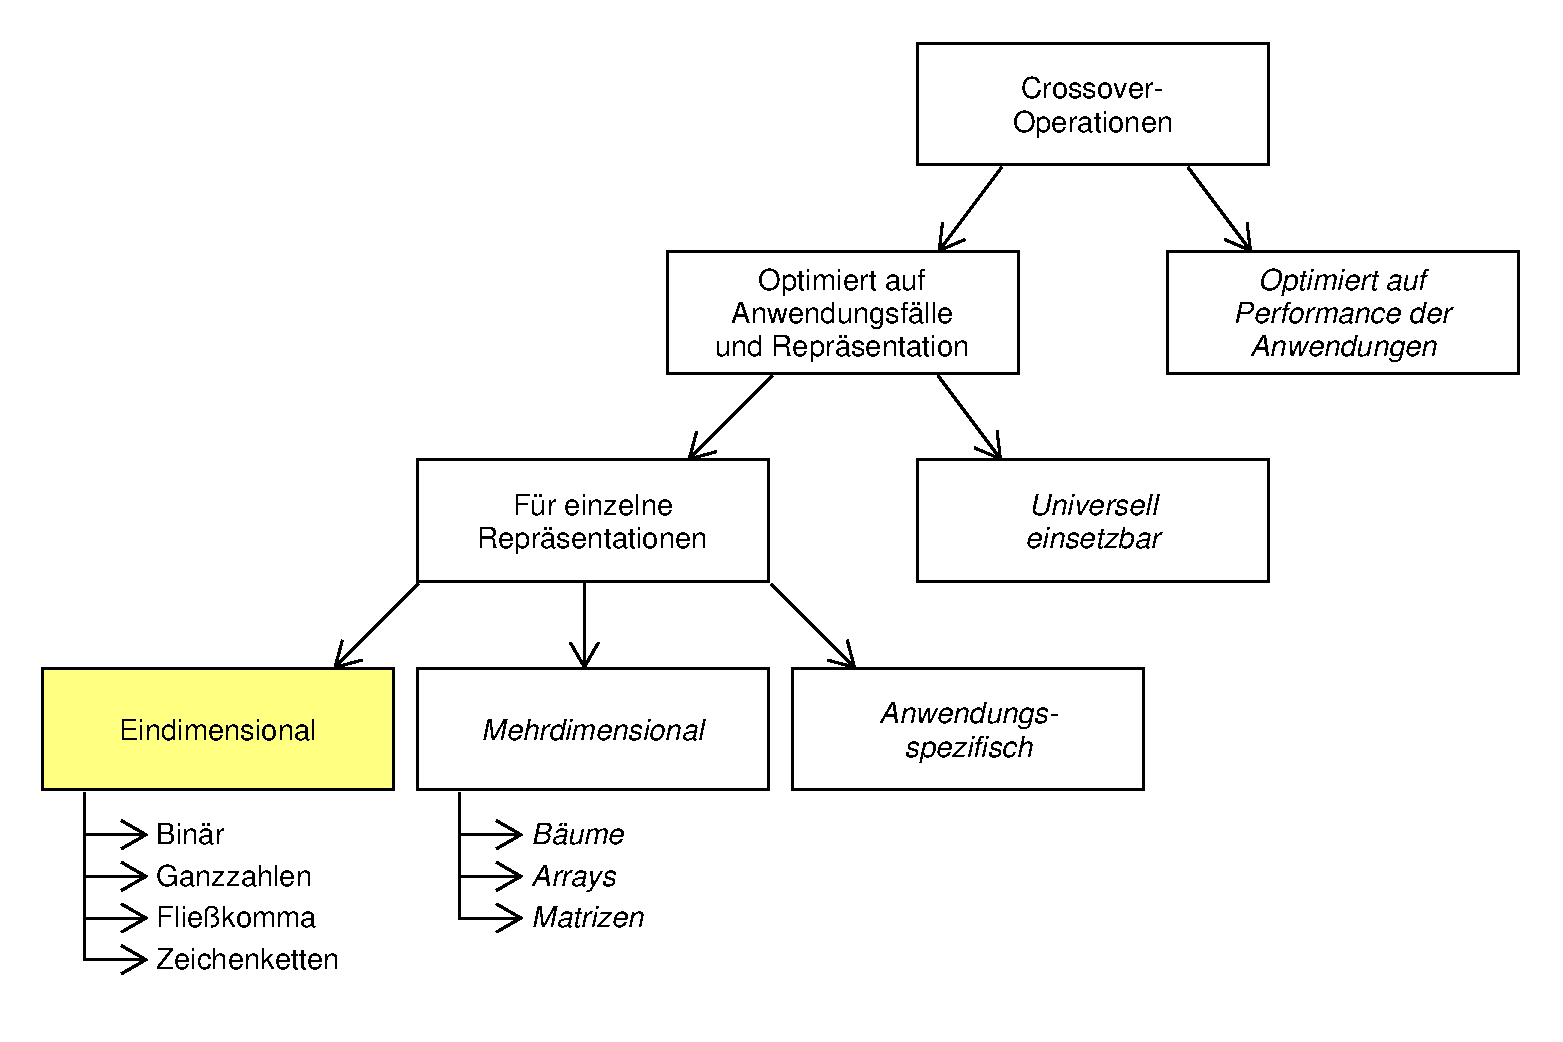
\includegraphics[width=.8\columnwidth]{./Figures/Crossover-Klassifizierung.pdf}
	\caption{Übersicht der Klassifizierung (nach \cite{Survey})}
	\label{fig:abb2}
\end{figure}

COs gibt es für viele verschiedene Arten von Anwendungen und Daten. Jedoch sind nicht alle möglichen Operationen für jede Anwendung und Daten\-art ge\-ei\-gnet. Pavai und Geetha haben daher in \cite{Survey} bereits einen sehr umfassenden Überblick über die verschiedenen Arten von COs gegeben, weshalb sich diese Seminararbeit an deren Arbeit orientiert. COs können, wie in Fig. \ref{fig:abb2} dargestellt, in verschiedenen Kategorien klassifiziert werden. Diese Arbeit befasst sich hauptsächlich mit eindimensionalen Darstellungsformen der Daten und deren entsprechenden COs. Für die kursiv markierten Klassifizierungen wird daher nur ein kurzer Überblick bzw. im Falle der performance-optimierten COs darauf verzichtet.

Die Basis aller verschiedenen COs bilden die elementaren Operationen, wel\-che die Gene der beiden Eltern an einer oder mehreren Stellen teilen und daraus die neuen Kinder erzeugen. Entsprechend werden sie auch \textit{N-Point-Crossover} bzw. im Speziellen auch \textit{One-Point-Crossover} oder \textit{Two-Point-Crossover} ge\-nannt. Darauf basierend gibt es noch weitere Basis-Operationen, wie \textit{Segmented Cross\-over}, bei der die Gene in eine bestimmte Anzahl Segmente anstatt an einer bestimmten Anzahl an Stellen geteilt werden, \cite{GABasicIdeas} oder wie \textit{Uniform Crossover}, bei der für jede Stelle des Kindes zufällig ausgewählt wird, welcher Elternteil sein Gen vererbt.

% !TEX root = main.tex

\section{Eindimensionale Repräsentation}
\label{sec:EindimRep}

Unter eindimensionaler Repräsentation wird vor allem die Darstellung der Daten in den elementaren Datentypen verstanden. Die Daten liegen dabei nur linear in einer bestimmten Reihenfolge vor, wodurch die Handhabung mit den Daten auch entsprechend einfach ist und in vielen Anwendungsfällen ohne große Probleme durchgeführt werden kann und entsprechend oft genutzt wird.

Zuerst wird im Abschnitt \ref{sec:BinCod} ein Überblick über Anwendungsfälle und mög\-liche COs für die Binär-Codierung gegeben. Anschließend wird in Abschnitt \ref{sec:IntCod} auf ganzzahlige Codierung allgemein bzw. auf Permutationen im Speziellen eingegangen, in Abschnitt \ref{sec:FloatCod} folgen Fließkomma-Darstellungen sowie in \ref{sec:StrCod} Zeichenketten.

\subsection{Binäre Codierung}
\label{sec:BinCod}

	Eine Codierung als Binärwerte bedeutet, dass die Werte, die vom GA bearbeitet werden, als eine Kette von 0 und 1 dargestellt sind. Der große Vorteil einer binären Codierung liegt vor allem darin, dass die Handhabung entsprechender Daten sehr einfach und platzsparend ist, weshalb diese Art der Darstellung prinzipiell von jeder Anwendung genutzt werden kann. Ebenfalls ein großer Vorteil liegt darin, dass entsprechende GAs aufgrund des geringen Alphabets sehr schnell und effizient sind.\cite{TacklingRealCodedGA}
	
	Vor allem folgende Arten von Anwendungen sind besonders dafür geeignet, mit binärer Codierung zu Arbeiten:\cite{Survey}
	\begin{description}
		\item[Classification Problem] Lösung soll in verschiedene Kategorien klassifiziert werden. \cite{NearestNeighborClassifier}
		\item[Multimodal Spin Lattice Problem] Suchen eines minimalen Ener\-gie\-zu\-stan\-des für 450 Spins mit je vier Zuständen auf einem 2D-Gitter. \cite{SelectionSchemesSpatialIsolation}
	\end{description}
	
	Passende Crossover-Operationen dafür sind:
	\begin{description}
		\item[Self-Crossover] Tauschen von einzelnen Bits innerhalb des Chromosoms. \cite{SelfCrossover}
		\item[Supplementary Crossover] Nutzt das \textit{Center of Gravity}-Paradigma um Kin\-der zu erzeugen. \cite{SupplementaryCrossover}
		\item[Generalized crossover] Interpretiert Chromosom als Ganzzahl und dividiert diese durch eine andere, zufällig ausgewählte Ganzzahl. \cite{GeneralizedCrossover}
	\end{description}

\subsection{Codierung als Ganzzahlen und Permutationen}
\label{sec:IntCod}

	Da ganzzahlige Werte ebenfalls sehr einfach als Binärwerte dargestellt werden können, können COs für Binärwerte prinzipiell auch für ganzzahlige Werte eingesetzt werden. Natürlich gibt es auch entsprechende Anwendungsfälle und COs, die speziell für ganzzahlige Darstellungen geeignet und optimiert sind, auf die hier aber verzichtet wird und stattdessen auf Ketten von ganzzahligen Werten, also Permutationen, eingegangen wird.
	
	Der Unterschied zwischen einfacher ganzzahligen Darstellungen und Permutationen liegt darin, dass bei Permutationen die komplette Zahlenfolge als mehrere aneinandergereihte Zahlen betrachtet werden muss. Entsprechend kön\-nen nicht einfache COs für Binärwerte und einfache ganzzahlige Werte eingesetzt werden, sondern COs, welche die Zahlenketten entsprechend berücksichtigen. Dies ist \uA bei folgenden Anwendungen und Problemen der Fall:
	\begin{description}
		\item[Traveling Salesman Problem (TSP)] Mehrere Orte, die mit einer möglichst kurzen Strecke miteinander verbunden werden müssen. \cite{GAforTSP}
		\item[Graph Coloring Problem] Knoten eines Graphen mit möglichst wenig und verschiedenen Farben einfärben. \cite{OrderBasedForGCP}
		\item[Quadratic Assignment Problem] Summe der Distanzen zwischen Punkten minimieren, ähnlich wie TSP, nur mit quadratischer Kostenfunktion. \cite{COforQAP}
	\end{description}
	
	Passende COs für Permutationen lassen sich in verschiedene Kategorien einteilen, welche sich basierend auf dem grundlegenden Vorgehen der COs klassifizieren lassen. Im Folgenden werden nun einige positionsbasierte, kantenbasierte und folgenbasierte COs vorgestellt. Daneben gibt es aber auch noch weitere, wie \zB teilmengenbasierte, die auf Basis von Genom-Teilmengen arbeiten, \textit{Cut and Splice}-basierte, die einen Teil der Elterngenome tauschen, oder distanzbasierte COs, bei denen die Anzahl der unterschiedlichen Gene zwischen allen Elternteile gleich sein muss.
	
	\subsubsection{Positionsbasierte COs}
	
		In dieser Kategorie finden sich vor allem COs, welche positionsbasiert einzelne Gene beeinflussen. Dies sind \uA folgende:
		
		\begin{description}
			\item[Partially Mapped Crossover (PMX)] Wählt zufällig zwei Punkte aus und tauscht alle Werte dazwischen mit dem anderen Elternteil. Bei der Er\-wei\-ter\-ung Uniform PMX werden einzelne Gene anstatt eines ganzen Segments getauscht. \cite{GAforTSP}\cite{COforPermutations}\cite{COforQAP}
			\item[Position Based Crossover (POS)] Wählt einige zufällige Positionen im ersten Elternteil aus und verschiebt die ausgewählten Werte zu den korrespondierenden Positionen im anderen Elternteil. \cite{COforPermutations}
		\end{description}
		
	\subsubsection{Kantenbasierte COs}
	
		In dieser Kategorie finden sich COs, welche basierend auf den Kanten der Eltern(-knoten) neue Kinder erzeugen. Darunter fallen \uA folgende COs:
		
		\begin{description}
			\item[Edge Crossover] Wählt einen Knoten mit der geringsten Kantenzahl aus und fügt ihn zum neuen Kind hinzu und löscht ihn aus den anderen Kantenlisten. \cite{COforPermutations}
			\item[Edge Exchange Crossover (EXX)] Vererbt zunächst alle Elternkanten um einen Kreis zu bilden, entfernt dann aber ungültige Kanten. Falls kein Kreis gebildet werden konnte, werden alle Kanten vererbt. \cite{EdgeCOforTSP}
		\end{description}
	
	\subsubsection{Folgenbasierte COs}
	
		Folgenbasierte COs beeinflussen vor allem die Reihenfolge der Gene. Sie lassen sich in weitere Unterkategorien einteilen. Darunter fallen \uA folgende COs:
		
		\begin{description}
			\item[Merging Crossover (MOX)] Beide Eltern werden zuerst zufällig zu\-sam\-men\-ge\-fügt und anschließend in die beiden Kinder geteilt. \cite{OrderBasedForGCP}
			\item[Non-Wrapping Ordered Crossover] Erstellt Lücken und füllt diese wieder auf, ohne dabei die absolute Reihenfolge der Gene zu verliern. \cite{GAforTSP}
		\end{description}
	
		Daneben gibt es auch noch weitere COs, welche sich neben den hier vorgestellten Unterkategorien (verschmelzende und absolute Reihenfolge) \zB in sor\-tier\-ende oder angrenzende, folgenbasierte COs einsortieren lassen.


\subsection{Codierung als Fließkommazahl}
\label{sec:FloatCod}

	Im Gegensatz zur Codierung als Ganzzahlen bzw. Binärwerte lassen sich Daten, welche als Fließkommazahlen codiert sind, viel genauer Darstellen, haben da\-durch aber auch einen deutlich größeren Suchraum für mögliche Lösungen. Dennoch liegt gerade darin der Vorteil, da die Art der Datencodierung möglichst mit der Codierung des Suchraumes übereinstimmen sollte. Dadurch entfällt die notwendige Konvertierung der Daten, wodurch letztlich die Geschwindigkeit und damit die Effizienz des GAs deutlich erhöht wird. Ebenso ist von Vorteil, dass große Suchräume mit kontinuierlichen Daten auf einfache Art und Weise abgesucht werden können anstatt lediglich mit diskreten Daten wie bei der Binärcodierung. \cite{TacklingRealCodedGA}
	
	Entsprechend lassen sich vor allem Anwendungen bzw. Probleme, welche einen kontinuierlichen Suchraum besitzen, mit Fließkomma-Codierungen effizient ausführen. Darunter fallen \zB folgende Anwendungen und Probleme:
	
	\begin{description}
		\item[Animal Diet Formulation Problem] Erstellung eines Ernährungsplans mit möglichst vielen Nährstoffen zu minimalen Kosten. \cite{ConceptOfCOInRealCoded}
		\item[Electromagnetic Optimization] Handhabung und Optimierung von elektromagnetischen Werten in einem kontinuierlichem Suchraum. \cite{ElectromagneticRealEncoding}
		\item[Revenue Management in Airlines] Zuweisen von begrenzten Ressourcen ei\-ner Airline (Flugzeuge, Personal, ...), um den Gewinn zu maximieren. \cite{AirlineRevenueManagement}
	\end{description}
	
	Als Fließkommazahlen codierte Daten kann man auf mehrere Arten verarbeiten, mit deren Basis die COs funktionieren. Dies sind \zB folgende Arten bzw. COs:
	
	\begin{description}
		\item[Taguchi Crossover (TC)] Nutzt statistische Daten innerhalb einer Matrix um das beste Ergebnis zu finden \cite{TaguchiCrossover}
		\item[Average Crossover] Modifizierter \textit{One-Point-Crossover}, bei dem die Durchschnittswerte zwischen beiden Eltern anstatt den Elternwerten der einzelnen Gene genutzt werden \cite{ConceptOfCOInRealCoded}
		\item[Fuzzy Arithmetic Weighted Mean (FAWM)] Berechnet mithilfe der Fuzzy-Arithmetik die Werte der Kinder \cite{AirlineRevenueManagement}
	\end{description}
	
	Daneben gibt es aber auch noch einige weitere Arten wie \zB den gewichteten Durchschnitt oder dem \textit{Center of Mass Crossover (CMX)}, welcher den gleichnamigen Ansatz nutzt um mithilfe des Massenzentrums der Eltern neue Kinder zu erzeugen. \cite{MultiParentRecombination} Daneben kann man aber auch verschiedene COs nutzen, um die Kinder zu erzeugen.

\subsection{Codierung als Zeichenkette}
\label{sec:StrCod}

	String-Codierungen

 % Eindimensionale Rep

% !TEX root = main.tex

\section{Mehrdimensionale Repräsentation}
\label{sec:MehrdimRep}

	Neben den verschiedenen eindimensionalen Repräsentationen der Daten gibt es natürlich auch mehrdimensionale Repräsentationsarten. Damit sind nicht einfache lineare, sondern komplexere Datenstrukturen gemeint, die entsprechend komplizierter zu Handhaben sind. Da es aber auch Anwendungen gibt, die mehrdimensionale Daten verarbeiten, gibt es auch entsprechende COs, um solche Daten einfach verarbeiten zu können.
	
	\subsubsection{Arrays}
	\label{sec:Arrays}
	
		dürften wohl eine der einfachsten Arten der Mehrdimensionalen Re\-prä\-sen\-ta\-ti\-on\-en darstellen. Sie bilden nicht mehr als eine Verkettung von mehreren linearen Datensätzen. Diese Art der Codierung kann für verschiedene Probleme genutzt werden wie \zB das TSP oder die Suche nach pareto-optimalen Lösungen, bei denen nicht alle Zieleigenschaften optimal sein können.
		
		Die dazu passenden COs heißen \uA \textit{Orthogonal Array Based Crossovers}, von denen es zwei Versionen gibt. Die erste Version heißt \textit{Orthogonal Crossover} und erzeugt die Kinder, indem die Elterngene basierend auf den Kombinationen eines orthogonalen Array ausgewählt werden. Die zweite Version namens \textit{Main Effect Crossover}  wählt die Kindergene im orthogonalen Array dagegen basierend auf deren Effekte aus, wodurch Kinder mit den besten Haupteffekten der Eltern generiert werden. \cite{ArrayCrossover}
	
	\subsubsection{Weitere mehrdimensionale Repräsentationen}
	\label{sec:WeitereMehrdim}
	
		sind beispielsweise \textit{Bäume} oder \textit{Matrizen}, bei denen die Daten entsprechend strukturiert und aufgebaut sind. Beide Darstellungsarten lassen sich \uA auch durch ähnliche COs bearbeiten, wie \zB den \textit{Reijmers Crossover Operator}, welcher aus den Distanzen zwischen den einzelnen Baumknoten eine Distanzen-Matrix erstellt, und diese mit einer vom GA generierten \textit{Correction-Matrix} addiert. \cite{MatrixCO}

\section{Anwendungsspezifische Codierung der Daten}
\label{sec:AnwSpezCod}

	Natürlich muss man nicht immer eine der üblichen ein- oder mehrdimensionalen Repräsentationsformen nutzen, wenn man einen GA entwickeln möchte. Es gibt auch Anwendungsfälle wie \zB in der Robotik, \cite{GABook} bei denen es geeigneter ist, eine speziell für die Anwendung zugeschnittene und optimierte Daten-Codierung zu nutzen.
	
	Die einfachste Variante dafür ist eine Art hybride Codierung zu nutzen, bei der zwei lineare Darstellungsformen miteinander kombiniert werden. Aguilar-Ruiz et al. haben dies in ihrer Arbeit \cite{NaturalCoding} gemacht und diskrete und kontinuierliche Darstellungsformen miteinander kombiniert, unterscheiden ihre \textit{Natural Encoding} jedoch von anderen hybriden Codierungen. Dennoch funktioniert ihr dabei entwickelter GA für klassische hybride und die \textit{Natural Encoding}.
	
	Daneben gibt es aber noch zahlreiche weitere Möglichkeiten, die Daten anwendungsspezifisch zu codieren und zu Handhaben. Einige davon wären \zB \textit{Restricted Growth Function}-basierte Techniken und COs, \cite{RestrictedGrowthFunction} oder die Mög\-lich\-keit, Fuzzy-Logiken zu nutzen. \cite{FuzzyEncoding}

\section{Universale Crossover-Operationen}
\label{sec:UnivOp}

	Neben den in dieser Seminararbeit vorgestellten spezifischen Darstellungsformen und entsprechenden COs gibt es aber auch noch einige COs, welche nicht auf eine bestimmte Repräsentationsart beschränkt sind, sondern mehrere verschiedene auf gleiche Art und Weise bearbeiten und daraus neue Kinder erzeugen können. Dies trifft zwar auch auf alle elementaren COs wie die \textit{N-Point-Crossover} zu, aber auch auf zahlreiche weitere COs, wie \zB der in \cite{COforPermutations} erwähnte \textit{Sorted Match Crossover}. Diese CO basiert auf den Kosten bzw. Fitness der Eltern und erzeugt neue Kinder, indem er einen Teil eines teuren bzw. guten Elternteils mit einem Teil eines billigen bzw. schlechten Elternteils kombiniert.
	
	Ähnlich wie den \textit{Uniform Crossover Operator} gibt es aber auch noch weitere COs, bei denen die Gene der Eltern zufallsbasiert vererbt werden. Ziemlich ähnlich funktionieren so \zB der \textit{Box Crossover} bzw. \textit{Extended Box Crossover}, bei denen die Gene der Kinder zufällig aus denen der Elternteile ausgewählt werden, wobei letzterer einen größeren Suchraum nutzt. \cite{BoxCrossover}
	
	Zudem besteht auch noch die Möglichkeit, zwei vorhandene COs miteinander zu kombinieren, wobei hier eine aufeinanderfolgende oder eine voneinander unabhängige (hybride) Ausführung möglich ist. Ein Beispiel für eine CO, welcher zwei COs kombiniert wäre der \textit{Uniform Wise Crossover (UWX)}, welcher den \textit{Uniform Crossover} mit dem \textit{Parameter Wise Crossover} kombiniert. \cite{ElectromagneticRealEncoding}
	
	Alternativ können auch heuristische COs genutzt werden. Einer davon ist der \textit{Adaptive Crossover}, welcher die Fitness-Werte der Elterngene bei der Erzeugung neuer Kinder berücksichtigt. % Alle anderen Reps

\section{Zusammenfassung}
\label{sec:ZusFass}

	Neben den hier vorgestellten COs gibt es für alle Darstellungsformen und deren Kategorisierungen noch zahlreiche weitere COs, von denen aufgrund der Länge dieser Seminararbeit viele nicht mal im Ansatz erwähnt wurden bzw. konnten. Wie Anfangs erwähnt haben Pavai und Geetha in \cite{Survey} eine Umfassende Übersicht erstellt, die sich ebenfalls lohnt, wenn man auf der Suche nach einer passenden CO für seine Anwendung ist.
	
	Wovon abhängig, was passende Repräsentation ist? einordnende Bewertung

\bibliographystyle{splncs03} 
\bibliography{literature}

\begin{comment}
\subsection{Grundlagen}
Text zu Fig.~\ref{fig:abb1}. Siehe Formel~\ref{eq:mean}

\subsubsection{Advantages and Challenges}
Eine Subsubsection.


\begin{figure}
	\centering
	\subfloat[Beispielbild 1]{
\includegraphics[width=0.5\columnwidth]{./Figures/Organic-Computing.png}}
	\hfill
	\subfloat[Beispielbild 2]{
\includegraphics[width=0.5\columnwidth]{./Figures/Organic-Computing.png}}
	\caption{Zwei Beispielbilder.}
\end{figure}

\begin{equation}
\label{eq:mean}
\bar{e} = \frac{1}{N}\sum_{i=1}^N{\lvert f_i - x_i\rvert}
\end{equation}
\end{comment}

\end{document}
